\section{Gilbert's LU factorization for sparse matrix}
This section is based on \cite{Gilbert1988}.

\begin{defn}[Symbolic analysis]
    When solving problems for sparse matrix, it's usually 
    more efficient when working with a fixed datastructure. 
    \textit{Symbolic analysis} is such a precursor to the 
    numerical solution, it includes computations that 
    typically depend only on the nonzero pattern, not the 
    numerical values. This will give a nonzero pattern of the 
    solution, so we can use a fixed datastructure to 
    store it.
\end{defn}

\begin{defn}
    Graph theory is a fundamental tool in sparse matrix 
    techniques. Graph $G_\mA=(V,E)$ for an 
    $\mathbb{R}^{n\times n}$ sparse matrix $\mA$ is defined by 
    vertices $V=\{1,\ldots,n\}$, edges $E=\{i\rightarrow j:
    a_{ij}\neq 0\}$ or $E=\{i\rightarrow j:a_{ji}\neq 0\}$ which 
    depend on the problem. When the matrix is symmetric, the 
    graph can be undirected. 
\end{defn}

\subsection{Solution for sparse triangular systems}
\label{section::sparseLxb}
\begin{lem}
    \label{lem::dfs}
    When we solve $\mL\mx=\mathbf{b}$, where both $\mL$ and 
    $\mathbf{b}$ are sparse and $\mL$ is lower triangular, 
    we should first use symbolic analysis to find the nonzero 
    pattern of $\mx$. This can be done by a depth-first search 
    in $G_\mL$ start with $\{i:b_i\neq 0\}$ where 
    $E=\{i\rightarrow j:l_{ji}\neq 0\}$. 
\end{lem}
\begin{proof}
    Formally, we have the relation
    \begin{equation}
        \label{eq::xiequation}
        x_i=b_i-\sum_{j=1}^{i-1}l_{ij}x_j.
    \end{equation}
    Notice that we are doing symbolic analysis, so we assume 
    no zero is produced during numerical calculation. So 
    $b_i\neq 0$ or $x_j\neq 0\cap l_{ij}\neq 0$ means there is 
    at least one nonzero term in \eqref{eq::xiequation}, so 
    \begin{align*}
        &b_{i}\neq 0\Rightarrow x_i\neq 0,\\
        &x_j\neq 0\cap l_{ij}\neq 0\Rightarrow x_i\neq 0.
    \end{align*}

    Now, assume $b_i\neq 0$, then $x_i\neq 0$. For all 
    $\{j:l_{ji}\neq 0\}$, we have $x_j\neq 0$, which is 
    equivalent to find all nodes who has an edge start from 
    $i$. Continue this search so we can find all $x_k\neq 0$ 
    because $b_i\neq 0$, this is indeed a search in 
    $G_\mL$. Do this for all $\{i:b_i\neq 0\}$, then we 
    find the nonzero pattern of $\mx$. Usually, the search is 
    performed by depth-first search.
\end{proof}

\begin{exm}
    For example, when we have $\mL$ and $G_\mL$ as in Figure 
    \ref{fig::LGL}.
    \begin{figure}[H]
        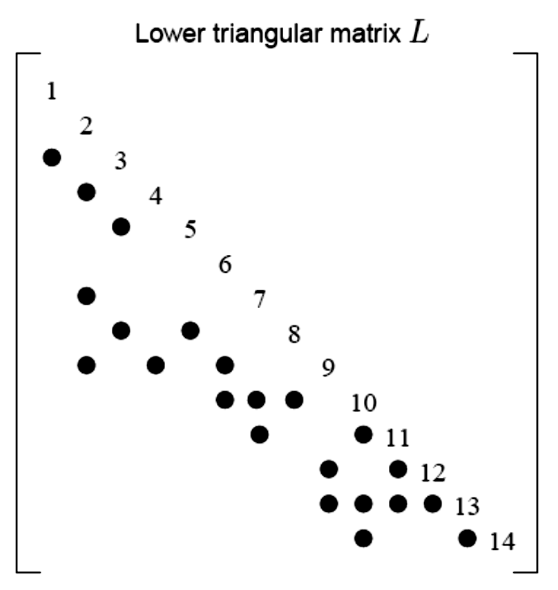
\includegraphics[width=0.49\linewidth]{png/L.png}
        \hfill
        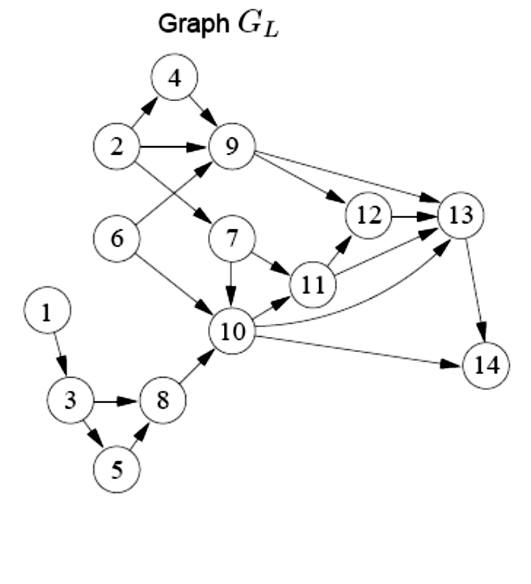
\includegraphics[width=0.49\linewidth]{png/GL.png}
        \caption{$\mL$ and corresponding $G_\mL$}
        \label{fig::LGL}
    \end{figure}
    Assuming only $b_4,b_6\neq 0$, then the depth-first 
    search paths are as in Figure \ref{fig::LGL2}, where the 
    red points in $\mL$ represent the edges in the search 
    paths.
    \begin{figure}[H]
        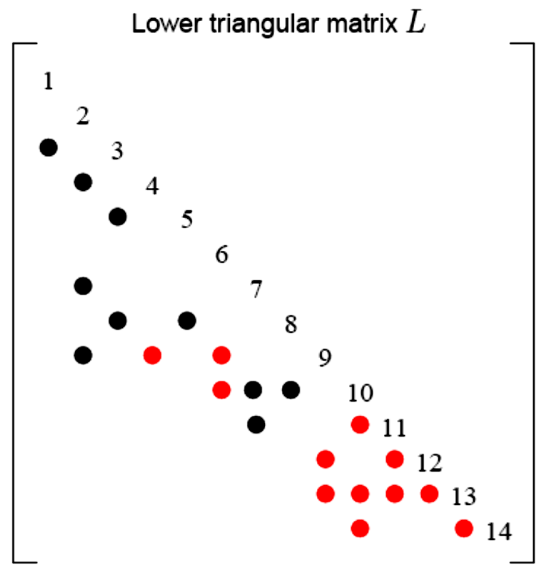
\includegraphics[width=0.49\linewidth]{png/L2.png}
        \hfill
        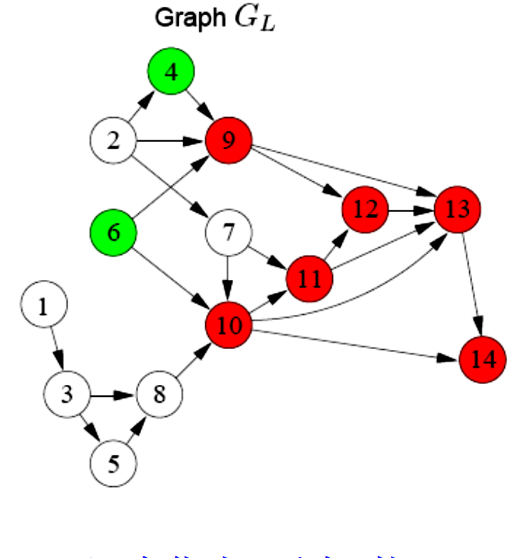
\includegraphics[width=0.49\linewidth]{png/GL2.png}
        \caption{The search paths of $\mL\mx=\mathbf{b}$}
        \label{fig::LGL2}
    \end{figure}
\end{exm}

\begin{lem}
    \label{lem::toporder}
    When we solve $\mL\mx=\mathbf{b}$ where $\mL$ is dense, we 
    use forward substitution, which would solve for the 
    unknowns in increasing order of row number. However, the 
    depth-first search may not find the nonzero positions of 
    $x_j$ in this order, and we don't want to sort it because 
    even a bucket sort would take $\mathcal{O}(n)$ time. 

    The solution to this problem is adding a stack during the 
    depth-first search, each time the depth-first search 
    backtracks from a vertex, that vertex is pushed into the 
    stack. After all the searches are done, the reverse order 
    of the stack is thus the order which will be used in 
    solving $x_j$, this order is also called the \textit{
    topological order}.
\end{lem}
\begin{proof}
    By \eqref{eq::xiequation}, we know that $x_i$ can be 
    calculated as soon as all the $\{x_k:l_{ik}\neq 0\cap 
    x_k\neq 0\}$ have been calculated. Notice that in the 
    depth-first search, if $l_{ik}\neq 0\cap x_k\neq 0$, 
    there must be an edge $k\rightarrow i$ in the search paths. 
    So, when the depth-first search backtracks from $i$, all 
    $\{k:l_{ik}\neq 0\cap x_k\neq 0\}$ are not in the stack 
    yet, otherwise there will be a contradiction. So when we 
    solve $x_i$ in the reverse order of the stack, we will 
    calculate all $\{x_k:l_{ij}\neq 0\cap x_k\neq 0\}$ before 
    we calculate $x_i$.
\end{proof}

\begin{thm}
    \label{thm::sparseLxbcost}
    The sparse lower triangular systems $\mL\mx=\mathbf{b}$ can 
    be solved in $\mathcal{O}(\mathrm{flops}(\mL\mx)+
    \eta(\mathbf{b}))$ time, where $\mathrm{flops}(\mL\mx)$ is 
    the number of multiplications of nonzeros when calculating 
    $\mL\mx$, $\eta(\mathbf{b})$ is the number of nonzeros in 
    $\mathbf{b}$.
\end{thm}
\begin{proof}
    There are two stages in solution, the depth-first search and 
    numerical calculation. The depth-first search takes time 
    proportional to the number of starting vertices plus the 
    number of edges traversed. The number of starting vertices 
    is obviously $\eta(\mathbf{b})$. The number of edges 
    traversed is the number of $\{(i,j):x_i\neq 0\cap 
    l_{ji}\neq 0\}$, notice that $(\mL\mx)_j=
    \sum_{\{i:x_i\neq 0\cap l_{ji}\neq 0\}}l_{ji}x_i$, so the 
    number of edges is exactly $\mathrm{flops}(\mL\mx)$. 

    As for the numerical calculation stage, since we know the 
    nonzero structure of $\mx$ before we start, we need only 
    initialize and manipulate the positions in the dense 
    vector that corresponding to nonzero positions, thus the 
    whole thing still takes only $\mathcal{O}(\mathrm{flops}
    (\mL\mx)+\eta(\mathbf{b}))$ time.
\end{proof}

\subsection{LU factorization with partial pivoting for sparse 
matrix}
\begin{alg}
    \label{alg::sparseLU}
    Since partial pivoting is used, we can't predict the 
    nonzero structure of the whole factors. \cite{Gilbert1988} 
    then compute the factors column by column just like the 
    left-looking LU factorization. Additionally, the 
    computation of each column of the factors is breaked into a 
    symbolic and numerical stage. Recall the procedure of 
    left-looking LU factorization with partial pivoting.
    \IncMargin{1em}
    %\LinesNumbered
    \begin{algorithm}[H]
        \caption{Left-looking LU factorization with partial 
        pivoting}
        \SetKwInOut{Precond}{Preconditions}
        \SetKwInOut{Postcond}{Postconditions}

        \KwIn{$\mA\in\mathbb{R}^{n\times n}$}
        \Precond{$\mA$ is nonsingular}
        \KwOut{$\mL,\mU\in\mathbb{R}^{n\times n}$}
        \Postcond{$\mL$ is unit lower triangular, $\mU$ is 
        upper triangular}

        \BlankLine
        $\mathbf{b}(1:n)=0$\;
        \For{$j=1:n$}{
            Solve $\mL(1:(j-1),1:(j-1))\mU(1:(j-1),j)=
            \mA(1:(j-1),j)$\;
            $\mathbf{b}(j:n)=\mA(j:n,j)-\mL(j:n,1:(j-1))
            \mU(1:(j-1),j)$\;
            Pivot: swap $b_{j}$ with the largest-magnitude 
            element of $\mathbf{b}(j:n)$, swap $\mL$ and $\mA$\;
            $u_{jj}=b_{j}$\;
            $\mL(j:n,j)=\mathbf{b}(j:n)/u_{jj}$\;
        }
    \end{algorithm}
    \DecMargin{1em}
    The left-looking LU factorization with partial pivoting 
    for sparse matrix is actually in the same form, excluding 
    the way to solve $\mL(1:(j-1),1:(j-1))\mU(1:(j-1),j)=
    \mA(1:(j-1),j)$. For sparse matrix, this lower triangular 
    systems can be solved just like what we have discussed in 
    Section \ref{section::sparseLxb}.
\end{alg}

\begin{thm}
    The entire algorithm \ref{alg::sparseLU} can be implmented 
    to run in $\mathcal{O}(\mathrm{flops}(\mL\mU)+\eta(\mA))$.
\end{thm}
\begin{proof}
    Define $m=\eta(\mA),\,m^*=\eta(\mL-\mI+\mU)$, then one can 
    show that $m^*-m\leq \mathrm{flops}(\mL\mU)$ because any 
    created nonzero element in $\mL-\mI+\mU$ is used in 
    $\mL\mU$ to balance other terms to make $\mL\mU=\mA$ hold. 
    
    By Theorem \ref{thm::sparseLxbcost}, step 2 and step 3 in 
    algorithm \ref{alg::sparseLU} take total time $\mathcal{O}
    (\mathrm{flops}(\mL\mU)+m^*)$ plus $\mathcal{O}(n)$ to 
    initialize the mark array for the depth-first search. Step 
    4 and step 6 each examine every nonzero in $\mL$ once, so 
    they take time $\mathcal{O}(m^*)$ over all. Step 5 takes 
    $\mathcal{O}(n)$ time overall. Since $n\leq m\leq m^*\leq 
    \mathrm{flops}(\mL\mU)+m$, the total is $\mathcal{O}
    (\mathrm{flops}(\mL\mU)+\eta(\mA))$.
\end{proof}